\section{Zielsetzung}

    \noindent In diesem Versuch wird wird ein Zusammenhang zwischen den Beugungsmuster, dem beugenden Objekt un der Aperturfunktion hergestellt.
    Dazu wird wird das Licht als Welle betrachtet nach dem es auf einen Spalt mit einem relativ zur Wellenlänge des Lichts kleine Abmessungen hat.

\section{Einleitung}

    \noindent Licht kann nicht mehr mittels geometrischen Optik betrachtet werden mehr dem es durch eine Öffnung hindurchtritt welche kleine 
    Abmessungen im Vergleich zur Wellenlänge des Lichts aufweist. Es entsteht Beugung, dieser Effekt lässt sich quantenmechanisch beschreiben, 
    es ist jedoch bei einer großen Anzahl an Lichtquanten, das Licht als Welle zu Nähern. 

\section{Theoretische Grundlagen}

    \noindent Zunächst wird zwischen der Fresnelschen und Fraunhoferschen Lichtbeugung unterschieden, diese sind in Abbildung(\ref{img:einzel}) 
    zu sehen. 

    \begin{figure}[ht]
        \centering
        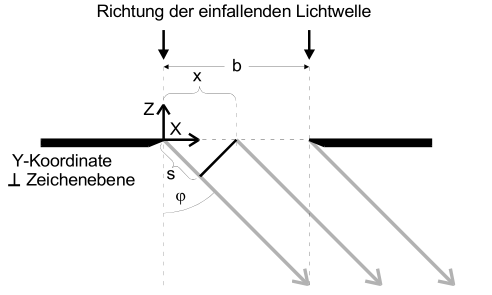
\includegraphics[width=0.5\textwidth]{latex/images/einzel.PNG}
        \caption{Fresnelsche und Fraunhofersche Beugung an einem Spalt\protect \cite{V406}.}
        \label{img:einzel}
    \end{figure}

    \noindent Bei der Fresnelschen Lichtbeugung am liegt die Lichtquelle in einer endlichen Entfernung vom Spalt und Beobachter, 
    damit nun zwei unterschiedliche Strahlenbündel an der gleichen Stelle auf dem Schirm ankommen, müssen sie am Spalt mit unterschiedlichen 
    Winkeln gebeugt werden. Bei der Frauenhoferschen Lichtbeugung liegt die Lichtquelle im unendlichen, so dass die eingehende Welle durch 
    eine ebene Welle beschreiben werden kann. Weiterhin werden die Strahl hinter dem Spalt durch eine Sammellinse gebündelt, somit wird 
    erreicht, dass die unterschiedlichen Lichtbündel die in Punkt P interferieren, mit dem gleichem Winkel gebeugt wurden. Der Parallelspalt 
    wird im folgenden mit der Frauenhofer Lichtbeugung betrachtet.

    \subsection{Parallelspalt}

        \noindent Hier wird ein Spalt mit hoher Länge im vergleich zur Breite genutzt, somit wird die Beugung auf eine Dimension beschränkt.
        Die Feldstärke der einfallenden ebenen Welle wird durch 

        \begin{equation*}
            A(z,t) = A_0 \text{exp}\left(i \omega t - \frac{i 2\pi z}{\lambda}\right)
        \end{equation*}

        \noindent beschrieben, mit der Zeit $t$ und dem Abstand in Z-Richtung $z$. Licht dieser Art kann mit einem Laser erstellt werden, 
        dieser liegt nicht in der unendlich großer Entfernung, sondern in einer Entfernung die groß im Vergleich zur Spaltbreite ist. 
        Das erscheinende Beugungsbild lässt sich mittels dem Huygenschen Prinzip der Elementarwellen und dem Interferenzprinzip 
        erklären. 
        
        
        
    

